\documentclass[tikz,border=5mm]{standalone}

\usepackage{tikz}
\usepackage{amsmath}
\usetikzlibrary{calc}

\begin{document}

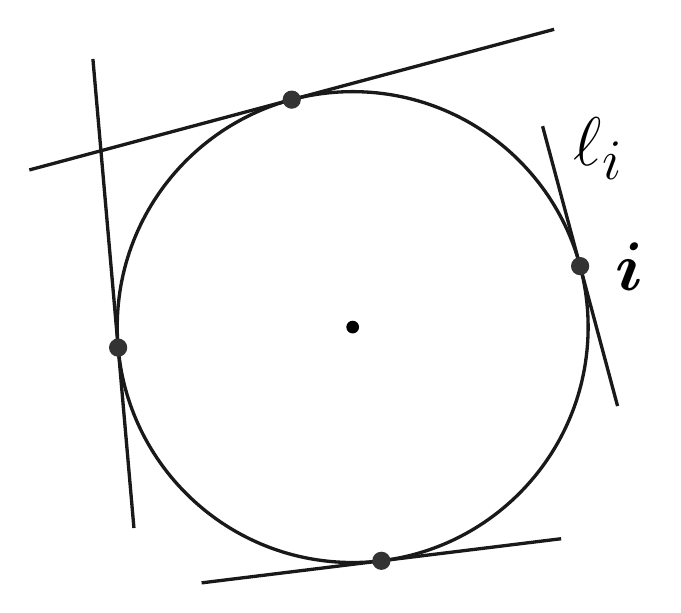
\begin{tikzpicture}[scale=1.15]

% ---------- parameters ----------
\def\R{2.6}
\def\angTop{15}
\def\angBot{7}
\def\angLeft{95}
\def\angRight{105}

% ---------- coordinates ----------
\coordinate (O)      at (0,0);
\coordinate (Ttop)   at ({\angTop+90}:\R);
\coordinate (Tbot)   at ({\angBot-90}:\R);
\coordinate (Tleft)  at ({\angLeft+90}:\R);
\coordinate (Tright) at ({\angRight-90}:\R);

% ---------- styles ----------
\tikzset{
  main/.style={draw=black!90,line width=1.2pt},
  dot/.style ={fill=black!80,draw=black!80,line width=0.6pt}
}

% ---------- circle ----------
\draw[main] (O) circle (\R);
\fill (O) circle (2pt);

% ---------- tangents ----------
% top (long)
\draw[main,rotate around={\angTop:(Ttop)}]
  ($(Ttop)+(-3,0)$) -- ($(Ttop)+(3,0)$);

% bottom (SHORTENED)
\draw[main,rotate around={\angBot:(Tbot)}]
  ($(Tbot)+(-2.0,0)$) -- ($(Tbot)+(2.0,0)$);

% left (unchanged)
\draw[main,rotate around={\angLeft:(Tleft)}]
  ($(Tleft)+(-2.0,0)$) -- ($(Tleft)+(3.2,0)$);

% right (SHORTENED)
\draw[main,rotate around={\angRight:(Tright)}]
  ($(Tright)+(-1.6,0)$) -- ($(Tright)+(1.6,0)$);

% ---------- contact points ----------
\fill[dot] (Ttop)   circle (2.6pt);
\fill[dot] (Tbot)   circle (2.6pt);
\fill[dot] (Tleft)  circle (2.6pt);
\fill[dot] (Tright) circle (2.6pt);

% ---------- labels ----------
\node at ($(Tright)+(0.55,0)$) {\fontsize{28}{32}\selectfont $\boldsymbol{i}$};

% larger l_s, moved left toward the circle
\node at ($(Tright)+(0.2,1.3)$) {\fontsize{32}{36}\selectfont $\ell_i$};

\end{tikzpicture}

\end{document}
